\documentclass[14pt,a4paper]{scrartcl}
\usepackage{cmap}
\usepackage[utf8]{inputenc}
\usepackage[T1,T2A]{fontenc}
\usepackage[english,russian]{babel}
\usepackage{relsize}
\usepackage{graphicx}
\usepackage{subfigure}
\usepackage{mathtools}
\usepackage{amssymb}
\usepackage{float}
\usepackage{sidecap}
\usepackage{wrapfig}
\usepackage{caption}
\usepackage[table,xcdraw]{xcolor}
\usepackage{listings}
\usepackage{amsmath,cryptocode}
\usepackage{listings}
\usepackage{booktabs}
\usepackage{multirow}  
\usepackage{multicol}
\usepackage{bigstrut}
\usepackage{lscape}
\usepackage{rotating}
\usepackage{adjustbox}
\usepackage{minted}
\usepackage{breqn}


\newcommand\scalemath[2]{\scalebox{#1}{\mbox{\ensuremath{\displaystyle #2}}}}


\begin{document}
	\begin{titlepage}
	\begin{center}
		\large
		МИНИСТЕРСТВО ОБРАЗОВАНИЯ И НАУКИ\\ РОССИЙСКОЙ ФЕДЕРАЦИИ
		
		\vspace{0.5cm}
		
		МГТУ им Н.Э.Баумана
		\vspace{0.25cm}
		
		Факультет ФН
		
		Кафедра вычислительной математики и математической физики
		\vfill
		
		
		Соколов Арсений Андреевич\\
		\vfill
		
		
		{\LARGE Лабораторная работа №5 по численным методам\\[2mm]
		}
		\bigskip
		
		3 курс, группа ФН11-53Б\\
		Вариант 6
	\end{center}
	\vfill
	
	\newlength{\ML}
	\settowidth{\ML}{«\underline{\hspace{0.7cm}}» \underline{\hspace{2cm}}}
	\hfill\begin{minipage}{0.4\textwidth}
		Преподаватель\\
		\underline{\hspace{3cm}} В.\,А.~Кутыркин\\
		«\underline{\hspace{0.7cm}}» \underline{\hspace{1.71cm}} 2019 г.
	\end{minipage}%
	\bigskip
	
	
	\vfill
	
	\begin{center}
		Москва, 2019 г.
	\end{center}
\end{titlepage}

\section*{Задание 1}
\textbf{Задание.}\\
Для гладкой на отрезке $[-1;1]$ функции $f(\tau) = \frac{10+0.5 \cdot N}{1+(20+0.25\cdot N)\cdot(1+0.05\cdot(53-n))\tau^2}$, $N$ -- номер фамилии студента в журнале, $n$ -- номер группы), используя равномерную сетку с 21 узлом, вычислить интерполяционный полином Лагранжа. Используя равномерную сетку с 41 узлом, представить графики функции $f$ и вычисленного (с 21 равномерными узлами) интерполяционного полинома Лагранжа. Прокомментировать результаты интерполяции.
Для гладкой на отрезке $[-1;1]$ функции $f$, используя чебышёвскую сетку с 21 узлом, вычислить интерполяционный полином Лагранжа. Используя равномерную сетку с 41 узлом, представить графики функции f и вычисленного (с 21 чебышёвскими узлами) интерполяционного полинома Лагранжа.
Прокомментировать результаты интерполяций с равномерными и чебышёвскими
узлами


\textbf{Исходные данные.}\\
$N = 6, n = 53$

\begin{equation*}
f(\tau) = \frac{10+0.5 \cdot N}{1+(20+0.25\cdot N)\cdot(1+0.05\cdot(53-n))\tau^2} = \frac{13}{1+21.5\tau^2}
\end{equation*}

\textbf{Решение.}\\
Рассмотрим на отрезке $[-1;1]$ сетку $A = \left\langle \tau_0, \tau_1, \ldots, \tau_{20}\right\rangle $ с 21 узлом. Получаем: 
\begin{equation*}
	\resizebox{1\hsize}{!}
	{$A = \langle -1, - 0.9, - 0.8, - 0.7, - 0.6, - 0.5, - 0.4, - 0.3, - 0.2, - 0.1, 0, 0.1, 0.2, 0.3, 0.4, 0.5, 0.6, 0.7, 0.8, 0.9, 1 \rangle$},
\end{equation*}
где $\tau_0, \tau_1, \ldots, \tau_{20}$ -- узлы этой сетки, то есть $-1 \leq \tau_0 \leq \tau_1 \leq \ldots \leq  \tau_{20} \leq 1$. Кроме того, зафиксирована $A-$сеточная функция $f_A:A\rightarrow\mathbb{R}$, обозначаемая далее вектором $\prescript{>}{}{y} = \left[ y_0, y_1, \ldots, y_{20} \right> \in \prescript{>}{}{\underline{\mathbb{R}}^{21}}(A)$, где $y_0=f_A(\tau_0), y_1=f_A(\tau_1), \ldots, y_{20}=f_A(\tau_20)$ и $\prescript{>}{}{\underline{\mathbb{R}}^{21}}(A)$ -- нормированное пространство $A-$сеточных функций с чебышёвской нормой $||\cdot||$, для которой $||\prescript{>}{}{y}|| = \max{|y_0|, |y_1|, \ldots, |y_{20}|}$

Получим:
	\pagebreak
\begin{table}[]
	\centering
	$\prescript{>}{}{y} = 
	\begin{pmatrix}
		0.5777777778 \\
		0.7059462395 \\
		0.8807588076 \\
		1.127004768  \\
		1.487414188  \\
		2.039215686  \\
		2.927927928  \\
		4.429301533  \\
		6.989247312  \\
		10.69958848  \\
		13.00000000  \\
		10.69958848  \\
		6.989247312  \\
		4.429301533  \\
		2.927927928  \\
		2.039215686  \\
		1.487414188  \\
		1.127004768  \\
		0.8807588076 \\
		0.7059462395 \\
		0.577777777
	\end{pmatrix}$
\end{table}

Используя равномерную сетку с 21 узлом, вычислим интерполяционный полином Лагранжа: 
\begin{equation*}
	L_{20}(\tau)=\sum_{i=0}^{20} \frac{\Lambda_{A}(\tau)}{\left(\tau-\tau_{i}\right) \Lambda_{A}^{\prime}\left(\tau_{i}\right)} y_{i}
\end{equation*}

\begin{dmath*}
	 L_{20}(\tau)=13.0+ 2370300.0\,{\tau}^{20}+ 0.00012537\,{\tau}^{19}- 9235800.0\,{
		\tau}^{18}+ 0.0053407\,{\tau}^{17}+ 14994000.0\,{\tau}^{16}+ 0.0053663
	\,{\tau}^{15}- 13246000.0\,{\tau}^{14}- 0.0040532\,{\tau}^{13}+
	6989300.0\,{\tau}^{12}+ 0.0040929\,{\tau}^{11}- 2283400.0\,{\tau}^{10
	}- 0.00020839\,{\tau}^{9}+ 466120.0\,{\tau}^{8}- 0.000023060\,{\tau}^{
		7}- 59456.0\,{\tau}^{6}+ 0.0000030940\,{\tau}^{5}+ 4825.0\,{\tau}^{4}-
	0.00000016103\,{\tau}^{3}- 272.79\,{\tau}^{2}+ 0.00000000048084\,\tau
\end{dmath*}

Рассмотрим совмещённые графики изначальной функции $f(\tau)$ и вычисленного интерполяционного полинома Лагранжа на равномерной сетке с 21 узлом:
\begin{figure}[h]
	\centering{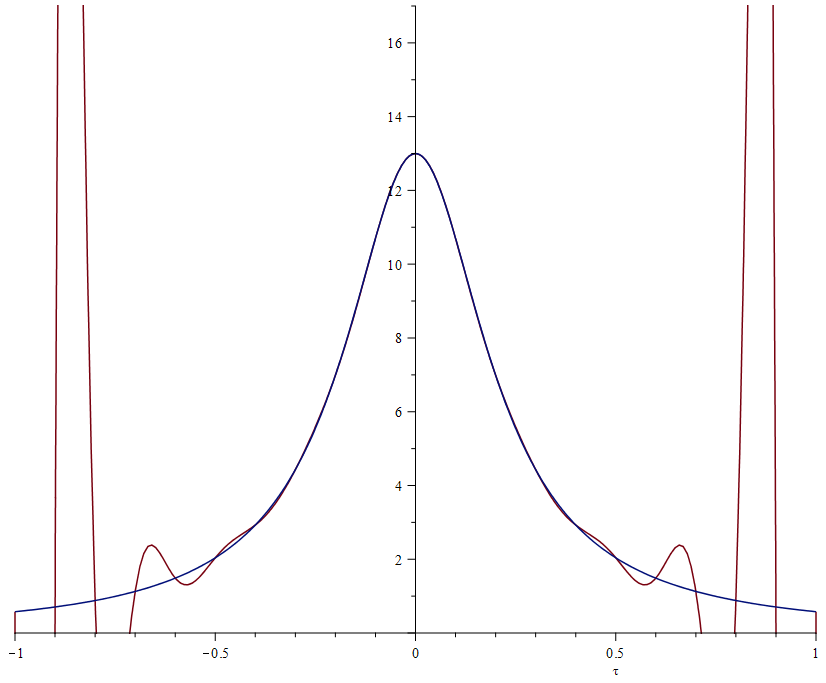
\includegraphics[width=0.9\linewidth]{../img/graph1.png}}
	\caption{Совмещённые графики функции $f(\tau)$ и вычисленного интерполяционного полинома Лагранжа на равномерной сетке с 21 узлом}
\end{figure}

\pagebreak

Теперь рассмотрим решение данной задачи с использованием чебышевской схемы сеток с 21 узлом:
\begin{equation*}
	A=\left\langle\tau_{j}=\frac{a+b}{2}-\frac{b-a}{2} \cdot \cos \frac{(2 j+1) \pi}{2(k+1)}: j=\overline{0, k}\right\rangle
\end{equation*}

Получим:
\begin{equation*}
	\begin{array}{l}{A=\left\langle-\cos \frac{\pi}{42},-\cos \frac{\pi}{14},-\cos \frac{5 \pi}{42},-\frac{\sqrt{3}}{2},-\cos \frac{3 \pi}{14},-\cos \frac{11 \pi}{42},-\cos \frac{13 \pi}{42},-\cos \frac{5 \pi}{14},-\cos \frac{17 \pi}{42}\right.} \\ {\left.-\cos \frac{19 \pi}{42}, 0, \cos \frac{19 \pi}{42}, \cos \frac{17 \pi}{42}, \cos \frac{5 \pi}{14}, \cos \frac{13 \pi}{42}, \cos \frac{11 \pi}{42}, \cos \frac{3 \pi}{14}, \frac{\sqrt{3}}{2}, \cos \frac{5 \pi}{42}, \cos \frac{\pi}{14}, \cos \frac{\pi}{42}\right\rangle}\end{array}
\end{equation*}

Соответствующая $A-$сеточная функция $f_A:A\rightarrow\mathbb{R}$, обозначаемая далее вектором $\prescript{>}{}{y} = \left[ y_0, y_1, \ldots, y_{20} \right> \in \prescript{>}{}{\underline{\mathbb{R}}^{21}}(A)$, где $y_0=f_A(\tau_0), y_1=f_A(\tau_1), \ldots, y_{20}=f_A(\tau_20)$ и $\prescript{>}{}{\underline{\mathbb{R}}^{21}}(A)$ -- нормированное пространство $A-$сеточных функций с чебышёвской нормой $||\cdot||$, для которой $||\prescript{>}{}{y}|| = \max{|y_0|, |y_1|, \ldots, |y_{20}|}$:

\begin{dmath*}
	\prescript{>}{}{y} = \left[ 0.642,0.67,0.732,0.839,1.017,1.315,1.843,2.865,5.076,10.001,\\
	15,10.001,5.076,2.865,1.843,1.315,1.017,0.839,0.732,0.67,0.642\right\rangle 
\end{dmath*}

Полином $\Lambda_A(\tau) = (\tau - \tau_0)\cdot(\tau - \tau_1)\cdot \ldots \cdot (\tau - \tau_{21})$, определённый на отрезке $[-1;1]$, называется $A-$сеточным полиномом.

Используя чебышёвскую сетку с 21 узлом, вычислим интерполяционный полином Лагранжа:
\begin{equation*}
L_{20}(\tau)=\sum_{i=0}^{20} \frac{\Lambda_{A}(\tau)}{\left(\tau-\tau_{i}\right) \Lambda_{A}^{\prime}\left(\tau_{i}\right)} y_{i}
\end{equation*}

Рассмотрим совмещённые графики изначальной функции $f(\tau)$ и вычисленного интерполяционного полинома Лагранжа на чебышёвской сетке с 21 узлом:
\begin{figure}[h]
	\centering{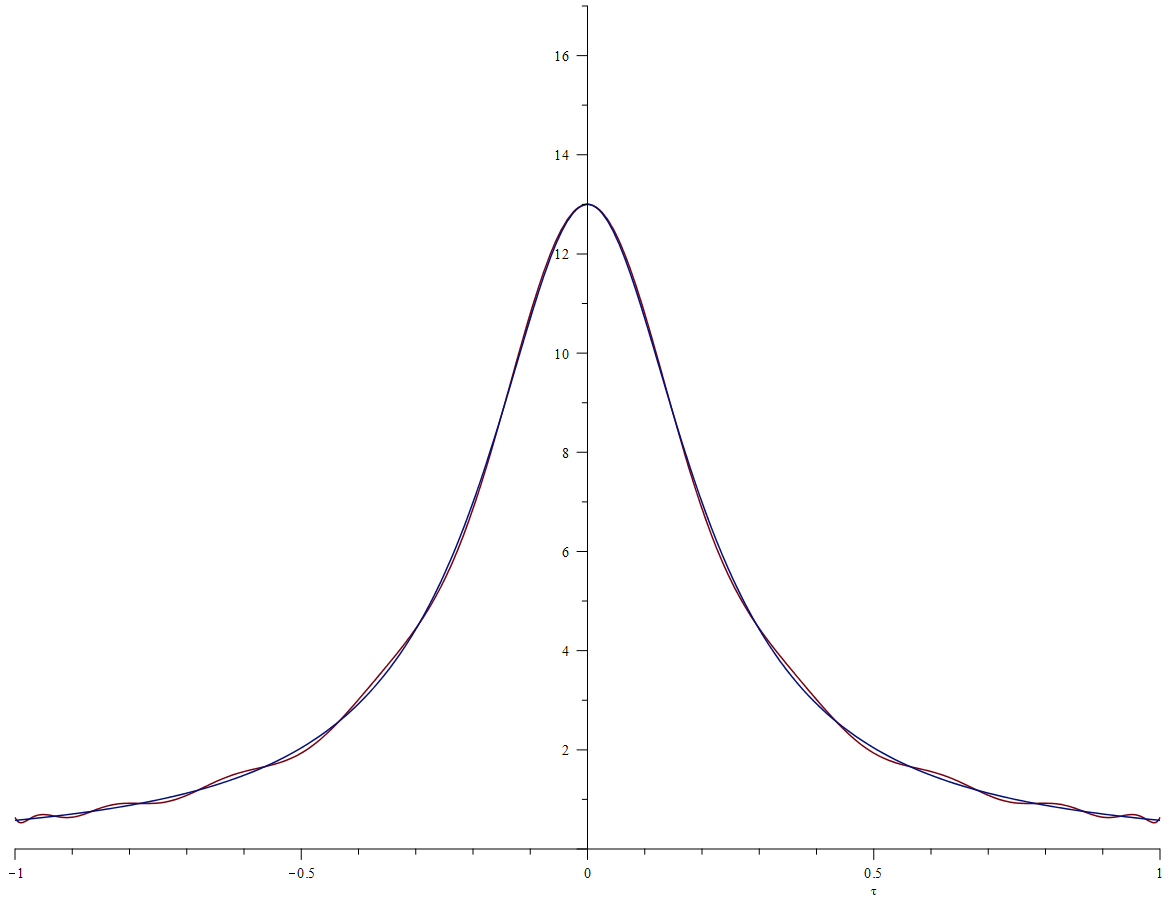
\includegraphics[width=0.9\linewidth]{../img/graph2.png}}
	\caption{Совмещённые графики функции $f(\tau)$ и вычисленного интерполяционного полинома Лагранжа на чебышёвской сетке с 21 узлом}
\end{figure}


\textbf{Выводы.}
Использование чебышёвской сетки при вычислении интерполяционного многочлена Лагранжа даёт лучшую аппроксимацию, чем равномерная сетка. При использовании равномерной сетки, отчелтиво видны выбросы на концах отрезка. 

\end{document}